\documentclass{beamer}

%%% ISSUE BBB solved %%%
%\usepackage{lmodern}
%%%%%%%%%%%%%%%%%%%%%%%%

\usepackage[utf8]{inputenc}
\usepackage[T1]{fontenc}
\usepackage{multicol}
\usepackage{amsthm}
\usepackage{amsmath}
\usepackage{amssymb}
\usepackage{mathtools}
\usepackage{dsfont}
\usepackage{bm}
\usepackage{bbm}
\usepackage{xparse}
\usepackage{physics}
\usepackage{empheq}
\usepackage{url}
\usepackage{hyperref}
%\usepackage[affil-it]{authblk}
%\usepackage{enumitem}
\usepackage{tikz}
\usetikzlibrary{quotes,angles,calc}
\usepackage{rotating}
\usepackage{graphicx}
\usepackage[linesnumbered,ruled,vlined]{algorithm2e}

\usepackage{pgfplots}
\pgfplotsset{compat = newest}

\theoremstyle{definition}
\newtheorem{theo}{Theorem}[section]
\newtheorem{lem}[theo]{Lemma}
\newtheorem{cor}[theo]{Corollary}
\newtheorem{prop}[theo]{Proposition}
\newtheorem{defi}[theo]{Definition}
\newtheorem{conj}[theo]{Conjecture}

\newtheorem{theo*}{Theorem}

\theoremstyle{remark}
\newtheorem*{rk}{Remark}

\DeclareMathOperator{\Poi}{\text{Poi}}
\DeclareMathOperator{\Ber}{\text{Ber}}
\DeclareMathOperator{\Bin}{\text{Bin}}
\DeclareMathOperator{\maxi}{\text{maximize}}
\DeclareMathOperator{\mini}{\text{minimize}}
\DeclareMathOperator{\st}{\text{subject to}}
\DeclarePairedDelimiter\ceil{\lceil}{\rceil}
\DeclarePairedDelimiter\floor{\lfloor}{\rfloor}
\DeclarePairedDelimiterX\set[1]\lbrace\rbrace{\def\given{\;\delimsize\vert\;}#1}

\colorlet{darkgreen}{green!40!black}

\usepackage{appendixnumberbeamer}


\usetheme{Dresden}
\usecolortheme{lily}
\newcommand*\oldmacro{}%
\let\oldmacro\insertshorttitle%
\renewcommand*\insertshorttitle{%
  \oldmacro\hfill%
  \insertframenumber\,/\,\inserttotalframenumber}


\title{Tight Approximation Guarantees for\\ Concave Coverage Problems}
\author{Siddharth Barman, Omar Fawzi, \textbf{Paul Fermé}}
\institute{arXiv:2010.00970}%\institute{LIP - ENS de Lyon}
\date{18/03/2021}

%\AtBeginSection[]
%{
%  \begin{frame}<beamer>
%    \frametitle{Contents}
%    \tableofcontents[currentsection]
%  \end{frame}
%}

%%%%%%%%%%%%%%%%%%%%%%%%%%%%%%%%%%%%%%%%%%
\begin{document}
%%%%%%%%%%%%%%%%%%%%%%%%%%%%%%%%%%%%%%%%%%

\begin{frame}
  \titlepage
\end{frame}

%%%%%%%%%%%%%%%%%%%%%%%%%%%%%%%%%%%%%%%%%%
\section{Introduction}


\begin{frame}{The \textsc{MaxCoverage} problem}
  \begin{columns}
    \begin{column}{5cm}
      \includegraphics<1,3->[scale=0.22]{MaxCovPlotNamed.png}%
      \includegraphics<2>[scale=0.22]{MaxCovPlotNamed1.png}%      
    \end{column}
    \begin{column}{5cm}
        \begin{align*}
          \maxi && C(S) := \abs{\bigcup_{i \in S} T_i}\\
          \st && \abs{S} = \only<1,3->{k} \only<2>{\alert{3}}
        \end{align*}
    \end{column}
  \end{columns}
  
  \bigskip
  \only<3->{
  \begin{itemize}
  \item NP-hard to approximate within a ratio $1 - e^{-1} + \varepsilon$ \cite{Feige98}.
  \item As $C$ is \emph{submodular}, the natural \emph{greedy} algorithm achieves the approximation ratio $1 - e^{-1}$ \cite{Hochbaum96}.
  \end{itemize}
  }
\end{frame}

\begin{frame}{A generalization}
  \begin{itemize}
  \item What happens if we take into account elements covered several times?
    \pause
    \bigskip
  \item \underline{Network coverage:}
    \begin{enumerate}
    \item \underline{$T_i$:} agents covered by antenna placement $i$.
    \item \underline{Goal:} find $k$ antenna locations maximizing coverage and bandwidth.
      \end{enumerate}
    \pause
  \item \underline{Multiwinner elections:}
    \begin{enumerate}
    \item \underline{$T_i$:} electors approving candidate $i$.
    \item \underline{Goal:} find  $k$ candidates maximizing the representative utility.
    \end{enumerate}

    \pause
    \bigskip

  \item The utility of an element covered $c$ times will be given by $\varphi(c)$.
  \item We suppose $\varphi$ nondecreasing concave and normalized, ie. $\varphi(0)=0$, $\varphi(1)=1$.
  \end{itemize}
\end{frame}

\begin{frame}%{Definition and examples}
    \begin{columns}
    \begin{column}{5cm}
      \includegraphics<1>[scale=0.20]{MaxCovPlotNamed.png}%
      \includegraphics<2>[scale=0.20]{MaxCovPlotNamed1.png}%
      \includegraphics<3>[scale=0.20]{MaxCovPlotNamed2.png}%
      \includegraphics<4>[scale=0.20]{MaxCovPlotNamed3.png}%

      \[ C^{\varphi}(\only<1>{S}\only<2>{\{3,4,5\}}\only<3>{\{1,2,5\}}\only<4>{\{2,3,5\}})=\only<1>{\ldots}\only<2>{\alert{9}}\only<3>{\alert{12}}\only<4>{\alert{11}} \]
    \end{column}
    \begin{column}{7cm}
        \begin{align*}
          \maxi &&& C^{\varphi}(S) := \sum_{a \in [n]}
          \only<1>{\varphi(\abs{S}_a)}
          \only<2>{\alert{\min\{\abs{S}_a,1\}}}
          \only<3>{\alert{\abs{S}_a}}
          \only<4>{\alert{\min\{\abs{S}_a,2\}}}\\
          \st &&& \abs{S} = \only<1>{k} \only<2->{\alert{3}}\\
          \text{with} &&& \abs{S}_a := \abs{\set{i \in S : a \in T_i}}
        \end{align*}
        \begin{center}
        \begin{tikzpicture}
          \draw[very thin,color=gray] (-0.1,-0.1) grid (3.1,3.1);
          \draw[->] (-0.2,0) -- (3.4,0) node[right] {$x$}; 
          \draw[->] (0,-0.2) -- (0,3.3) node[above] {$\varphi(x)$};
          \draw (0,0) node[below left] {$0$};
          \draw[color=red,thick] plot[domain=0:1,smooth] (\x,{\x});
          \only<1>{\draw[color=red,thick] plot[domain=1:3.1,smooth] (\x,{1+ln(\x)});}
          \only<2>{\draw[color=red,thick] plot[domain=1:3.1,smooth] (\x,{1});}
          \only<3>{\draw[color=red,thick] plot[domain=1:3.1,smooth] (\x,{\x});}
          \only<4>{\draw[color=red,thick] plot[domain=1:2,smooth] (\x,{\x});
            \draw[color=red,thick] plot[domain=2:3.1,smooth] (\x,{2});}
        \end{tikzpicture}
        \end{center}
    \end{column}
    \end{columns}

\end{frame}

\begin{frame}{Our results}
  \underline{$\varphi$-\textsc{MaxCoverage} problem:}
    \begin{align*}
      \maxi &&& C^{\varphi}(S) := \sum_{a \in [n]} w_a\varphi(\abs{S}_a)\\
      \st &&& \abs{S} = k
    \end{align*}

  \pause
  
  \begin{theo}[Main Result]
    There exists a polynomial-time approximation algorithm achieving the \emph{Poisson concavity ratio} of $\varphi$, defined by:
    \[ \alpha_{\varphi} := \min_{x \in \mathbb{N}^*} \alpha_{\varphi}(x) \text{, with } \alpha_{\varphi}(x) := \frac{\mathbb{E}[\varphi(\Poi(x))]}{\varphi(\mathbb{E}[\Poi(x)])}\ .\]
    Furthermore for $\varphi(n) = o(n)$, it is \textrm{NP}-hard to approximate within a better ratio than $\alpha_\varphi + \varepsilon$.
  \end{theo}
\end{frame}

\begin{frame}{Previous work}
  \begin{itemize}
  \item \cite{SVW17}: Generic algorithm for \emph{submodular} maximization using the \emph{curvature} $c$, ratio $1-ce^{-1}$.\\
  $\Rightarrow$ We have shown that $\alpha_{\varphi} \geq 1-ce^{-1}$, $c$ curvature of $C^{\varphi}$.
    \pause
    \bigskip
  \item \cite{BFGG20}: \underline{$\ell$-\textsc{MultiCoverage} problem:} $\varphi(j):=\min\{ j,\ell\}$, ratio $1-\frac{\ell^{\ell}e^{-\ell}}{\ell!}$, tight under UGC.\\
  $\Rightarrow$ One can compute $\alpha_{\varphi} = \alpha_{\varphi}(\ell) = 1-\frac{\ell^{\ell}e^{-\ell}}{\ell!}$, tight if \textrm{P}$\not=$\textrm{NP}.
    \pause
    \bigskip
  \item \cite{DMMS20}: For \emph{geometrically dominant} $\varphi$, ratio $\mathbb{E}[\varphi(\Poi(1))]$, tight if $\varphi(n) = o(n)$ and \textrm{P}$\not=$\textrm{NP}.\\
  $\Rightarrow$ We have shown that if $\varphi$ is geometrically dominant, then $\alpha_\varphi=\alpha_\varphi(1)=\mathbb{E}[\varphi(\Poi(1))]$.
  \end{itemize}
\end{frame}

\begin{frame}{Some particular cases}
  \begin{table}[!h]
  \begin{center}
    \begin{tabular}{|l|l|l|}
      \hline
      $\varphi$-\textsc{MaxCoverage}  & $\varphi(j)$ & $\alpha_{\varphi}$ \\
      \hline
      \textsc{MaxCoverage} & $\min \{ j,1\}$ & $1 - e^{-1}$  \\
      $\ell$-\textsc{MultiCoverage} & $\min\{ j,\ell\}$ & $1-\frac{\ell^{\ell}e^{-\ell}}{\ell!}$ \\
       \textsc{PAV} & $\sum_{i=1}^j \frac{1}{i}$ & $\alpha_{\varphi}(1) \simeq 0.7965\ldots$\\
      \textsc{PAV} capped at $3$ & $\sum_{i=1}^{\min\{j,3\}} \frac{1}{i}$ & $\alpha_{\varphi}(1) \simeq 0.7910\ldots$ \\
      $p$-\textsc{VTA} & $\frac{1-(1-p)^j}{p}$ & $\frac{1 - e^{-p}}{p}$  \\
      $0.1$-\textsc{VTA} & $\frac{1-(1-0.1)^j}{0.1}$ & $\frac{1 - e^{-0.1}}{0.1} \simeq 0.9516\ldots$ \\
      $0.1$-\textsc{VTA} capped at $5$ & $\frac{1-(1-0.1)^{\min\{j,5\}}}{0.1}$ & $\alpha_{\varphi}(5) \simeq 0.8470\ldots$  \\
      \hline
    \end{tabular}
  \end{center}
  \caption{Tight approximation ratios for particular choices of $\varphi$ in the $\varphi$-\textsc{MaxCoverage} problem.}
  \label{figComp}
\end{table}
\end{frame}

%%%%%%%%%%%%%%%%%%%%%%%%%%%%%%%%%%%%%%%%%%
\section{Approximation Algorithm}
\begin{frame}{Linear Relaxation of $\varphi$-\textsc{MaxCoverage}}
  \begin{itemize}
  \item \emph{Relax and Round} strategy to achieve the ratio $\alpha_{\varphi}$.
    \pause
  \item We consider $\varphi$ on $\mathbb{R}^+$, by extending it piecewise linearly:  
  \begin{align*}
      &\maxi&& \sum_{a \in [n]} w_ac_a \\
      &\st&& c_a \leq \varphi(\abs{x}_a), \forall a \in [n],\text{ with }\abs{x}_a := \sum_{i \in [m] : a \in T_i} x_i\\
      &&& 0 \leq x_i \leq 1, \forall i \in [m]\\
      &&& \sum_{i=1}^m x_i = k \ .
  \end{align*}
  \pause
  
\item Note that $c_a \leq \varphi(\abs{x}_a)$ equivalent to $c_a \leq \varphi_j(\abs{x}_a)$ for all $j \in [m]$, with $\varphi_j$ linear interpolation of $\varphi(j-1)$ and $\varphi(j)$.
  \end{itemize}
  
\end{frame}

\begin{frame}
  \begin{center}
    \includegraphics[scale=0.35]{PhiLinearConstraint.png}
  \end{center}
\end{frame}

\begin{frame}{Pipage Rounding}
  $C^{\varphi}$ \emph{submodular}: use \emph{pipage rounding} to get integral solution from fractional one.

  \pause
  
  \begin{defi}[Multilinear extension]
    The multilinear extension $F : [0, 1]^m \rightarrow \mathbb{R}$ of $f$ is defined by:\\
    $F(x_1,\ldots,x_m): = \mathbb{E}[f(X_1,\ldots,X_m)]$, $X_i \sim \Ber(x_i)$ independent.
  \end{defi}

  \begin{theo}[\cite{AS04, Vondrak07}]
    For $f$ submodular and $F$ computable in polynomial time, the \emph{pipage rounding} procedure applied on a fractional solution $x$ gives in polynomial time an integer solution $x^{\text{int}}$ with $F(x^{\text{int}}) \geq F(x)$.
  \end{theo}

  \bigskip
  \pause
  
  Applied to our setting, with $x^*$ an optimal fractional solution:
  \[C^{\varphi}(x^{\text{int}}) \geq \mathbb{E}_{X \sim \Ber(x^*)}[C^{\varphi}(X)]\ .\]
\end{frame}

\begin{frame}{Approximation Guarantee Theorem}
  \begin{theo}
      Let $x,c$ be a feasible solution of our linear relaxation and $X \sim \Ber(x)$. We have:
      \[\mathbb{E}_{X \sim \Ber(x)}[C^{\varphi}(X)] \geq \left(\min_{j \in [m]} \alpha_{\varphi}(j)\right) \sum_{a \in [n]} w_ac_a\ .\]
  In particular, this implies that the described polynomial time algorithm has an approximation ratio of $\alpha_{\varphi}$:
  \begin{align*}
    C^{\varphi}(x^{\text{int}}) &\underset{\text{Rounding}}{\overset{\text{Pipage}}{\geq}} \mathbb{E}_{X \sim \Ber(x^*)}[C^{\varphi}(X)]  \overset{\text{AGT}}{\geq} \alpha_{\varphi} \sum_{a \in [n]} w_ac^*_a\\
    &\underset{\text{Relax}}{\geq} \alpha_{\varphi} \max_{S \subseteq [m] : \abs{S} = k} C^{\varphi}(S)\ .
  \end{align*}
  \end{theo}
\end{frame}

\begin{frame}{Key lemma}
  \begin{lem}
    For $\varphi$ concave, and $p \in [0,1]^m$, we have $\mathbb{E}\Big[\varphi\Big(\sum_{i=1}^m\Ber(p_i)\Big)\Big] \geq \mathbb{E}\Big[\varphi\Big(\Poi\Big(\sum_{i=1}^m p_i\Big)\Big)\Big]$.    
    \label{lem:ConvexOrder}
  \end{lem}

  
  \bigskip
  \pause

  \begin{itemize}
  \item Notion of \emph{convex order} used to prove this result: $X \leq_{\text{cx}} Y \iff \mathbb{E}[f(X)] \leq \mathbb{E}[f(Y)]$ for any convex $f$.
    \pause
    \item We have $\forall p_i \in [0,1], \Ber(p_i) \leq_{\text{cx}} \Poi(p_i)$.
    \item Convex order is preserved through convolution.
    \item $\sum_{i=1}^m \Poi(p_i) \sim \Poi\Big(\sum_{i=1}^m p_i\Big)$. So:
      \[\sum_{i=1}^m\Ber(p_i) \leq_{\text{cx}}  \Poi\Big(\sum_{i=1}^m p_i\Big)\ .\]
      \pause
\item Apply this to convex $-\varphi$.
  \end{itemize}
\end{frame}

%%%%%%%%%%%%%%%%%%%%%%%%%%%%%%%%%%%%%%%%%%
\section{Applications}
\begin{frame}{Resource Allocation in Multiagent Systems}
  \begin{itemize}
  \item \underline{Algorithmic game theory:} maximizing welfare among multiple agents \cite{PM19}.
    
  \item \underline{$\varphi$-\textsc{Resource Allocation} problem:}
    \begin{enumerate}
    \item $n$ resources,
    \item $k$ agents,
    \item agent $i$ has resources $\mathcal{A}_i = \set{T^i_1, \ldots, T^i_{m_i}}$, with $T^i_j \subseteq [n]$,
    \item a counting function $\varphi: \mathbb{N} \rightarrow \mathbb{R}_+$,
    \end{enumerate}
    
    \underline{Goal:} maximize $W^{\varphi}(A_1, A_2, \ldots, A_k)  \coloneqq \sum_{a \in [n]} w_a \ \varphi(\abs{A}_a)$ with  $A_i \in \mathcal{A}_i$ and $\abs{A}_a \coloneqq  \abs{\set{i \in [k] : a \in A_i}}$.

    \pause
    \bigskip
  \item $\varphi$-\textsc{Resource Allocation} is a $\varphi$-\textsc{MaxCoverage} instance subject to a \emph{partition matroid} constraint.
  \item With adapted hardness proof, we get the same theorem as for $\varphi$-\textsc{MaxCoverage}.
  \end{itemize}
\end{frame}

\begin{frame}{An example: \textsc{Vehicle-Target Assignment}~\cite{Murphey00}}
  \begin{itemize}
  \item Particular case of $\varphi$-\textsc{Resource Allocation}:
    \begin{enumerate}
    \item resources correspond to targets $[n]$,
    \item agents correspond to vehicles $[k]$,
    \item vehicle $i$ has several possible assignments, described as target covering sets $\mathcal{A}_i \subseteq 2^{[n]}$,
    \item $\varphi^p(j) = \frac{1-(1-p)^j}{p}$, for some $p \in (0,1)$.
    \end{enumerate}
    \pause
    \bigskip
  \item $\varphi^p$ is nondecreasing concave and $\varphi(n)=o(n)$: we get the tight ratio $\alpha_{\varphi^p} = \frac{1 - e^{-p}}{p}$.
    \bigskip
  \item Capped version of this problem: $\varphi^p_{\ell}(j) := \varphi^p(\min\{j,\ell\})$.\\In particular, we recover the $\ell$-\textsc{MultiCoverage} function when $p=0$ and \textsc{MaxCoverage} for $p=1$.
  \end{itemize}
  
\end{frame}

\begin{frame}
  
\begin{figure}[!h]
  \begin{center}
    \begin{tikzpicture}
      \begin{axis}[
          xmin = 0, xmax = 1,
          ymin = 0.5, ymax = 1,
          xtick distance = 0.2,
          ytick distance = 0.1,
          grid = both,
          width = 0.95\textwidth,
          height = 0.55\textwidth,
          legend cell align = {left},
          legend pos = north east,
          xlabel=$p$,
        ]
        \addplot[
          domain = 0:1,
          samples = 21,
          smooth,
          black,
          mark = x,
        ] table[x=p,y=alpha,col sep=comma] {VTATruncPlot.csv};
        \addplot[
          domain = 0:1,
          samples = 21,
          smooth,
          brown,
          mark = triangle,
        ] table[x=p,y=m1,col sep=comma] {VTATruncPlot.csv};
        \addplot[
          domain = 0:1,
          samples = 21,
          smooth,
          orange,
          mark = o,
        ] table[x=p,y=m2,col sep=comma] {VTATruncPlot.csv};
        \addplot[
          domain = 0:1,
          samples = 21,
          smooth,
          purple,
          mark = diamond,
        ] table[x=p,y=m3,col sep=comma] {VTATruncPlot.csv};
        \addplot[
          domain = 0:1,
          samples = 21,
          smooth,
          red,
          mark = square,
        ] table[x=p,y=m4,col sep=comma] {VTATruncPlot.csv};
        \addplot[
          domain = 0:1,
          samples = 21,
          smooth,
          blue,
          mark = star,
        ] table[x=p,y=m5,col sep=comma] {VTATruncPlot.csv};

        \legend{$\alpha_{\varphi^p_{\infty}}$, $\alpha_{\varphi^p_{1}}$, $\alpha_{\varphi^p_{2}}$, $\alpha_{\varphi^p_{3}}$, $\alpha_{\varphi^p_{4}}$, $\alpha_{\varphi^p_{5}}$ }
      \end{axis}
    \end{tikzpicture}
  \end{center}
  \caption{Tight approximation ratios $\alpha_{\varphi^p_{\ell}}$, where $\ell$ is the rank of the capped version of the $p$-\textsc{Vehicle-Target Assignment} problem. When $p=0$, we recover the $\ell$-\textsc{MultiCoverage} problem.}
  \label{fig:VTATrunc}
\end{figure}
\end{frame}

\begin{frame}{Links to \emph{Price of Anarchy}}
  \begin{itemize}
  \item \cite{PM19}: game-theoretic aspects of $\varphi$-\textsc{Resource Allocation} problem, and in particular \textsc{VTA}.
  \item \underline{Goal:} bound welfare loss due to self-interested choice of $A_i \in \mathcal{A}_i$ by each agent $i$, defined as the \emph{Price of Anarchy}.
  \item In that setting, the PoA can be computed via linear programs. 

    \pause
    \bigskip

  \item \underline{Our hardness result} $\Rightarrow$ upper bounds on those PoA.
  \item \cite{CPM19}: in the particular case of the $\ell$-\textsc{MultiCoverage} problem, PoA $=\alpha_{\varphi}$.
  \item However, numerically comparing $\alpha_{\varphi}$ for \textsc{VTA} with the optimal PoA bound,  $\alpha_{\varphi}$ can in fact be strictly greater than the PoA guarantee.
  \end{itemize}
\end{frame}

\begin{frame}
\begin{figure}[!h]
      \begin{center}
       \begin{tikzpicture}
          \begin{axis}[
            xmin = 0, xmax = 1,
            ymin = 0.5, ymax = 1,
            xtick distance = 0.2,
            ytick distance = 0.1,
            grid = both,
            width = 0.95\textwidth,
            height = 0.55\textwidth,
            legend cell align = {left},
            legend pos = north east,
            xlabel=$p$,
            ]
            \addplot[
              domain = 0:1,
              samples = 21,
              smooth,
              black,
              mark = x,
            ] table[x=p,y=alpha,col sep=comma] {VTAPoA.csv};
            \addplot[
              domain = 0:1,
              samples = 21,
              smooth,
              blue,
              mark = o,
            ] table[x=p,y=PoA,col sep=comma] {VTAPoA.csv};
            \addplot[
              domain = 0:1,
              samples = 21,
              smooth,
              red,
              mark = diamond,
            ] table[x=p,y=App,col sep=comma] {VTAPoA.csv};
            \legend{$\alpha_{\varphi^p} = \frac{1 - e^{-p}}{p}$, PoA$^{20}$,Curv $=1 - \frac{c}{e}$}
          \end{axis}
       \end{tikzpicture}
    \end{center}
    \caption{Comparison between the PoA and $\alpha_{\varphi}$ for the \textsc{Vehicle-Target Assignment} problem. Since the PoA only decreases when the number of players grows, this means that PoA $< \alpha_{\varphi}$ in that case.}
    \label{fig:VTA}
\end{figure}
\end{frame}

%%%%%%%%%%%%%%%%%%%%%%%%%%%%%%%%%%%%%%%%%%
\appendix
%%%%%%%%%%%%%%%%%%%%%%%%%%%%%%%%%%%%%%%%%%
\section{Conclusion}
\begin{frame}{Conclusion and Open Questions}
  \begin{itemize}
  \item $\varphi$-\textsc{MaxCoverage}: generalization of \textsc{MaxCoverage} where having $c$ copies of element $a$ gives a value $\varphi(c)$.
  \item For nondecreasing concave $\varphi$, approximation guarantee given by the \emph{Poisson concavity ratio} $\alpha_{\varphi} := \min_{x \in \mathbb{N^*}} \frac{\mathbb{E}[\varphi(\Poi(x))]}{\varphi(\mathbb{E}[\Poi(x)])}$.
  \item Tight for sublinear functions $\varphi(n)=o(n)$.
  \item Beats the curvature bound as soon as $\varphi(t)\not=1+(1-c)t$, where they are equal.

    \pause
    \bigskip
    
    \item Open questions:
      \begin{enumerate}
      \item Does there exist combinatorial algorithms that achieve $\alpha_{\varphi}$?
      \item Does the hardness result remain true when $\varphi(n) \not= o(n)$?
      \end{enumerate}
      \bigskip
      \pause
      \item Thank you for listening!
  \end{itemize}
\end{frame}

%%%%%%%%%%%%%%%%%%%%%%%%%%%%%%%%%%%%%%%%%%
\section{Bibliography}
\begin{frame}[allowframebreaks]{Bibliography}
  \bibliographystyle{apalike}
  \bibliography{MaxCoverage}
\end{frame}
%%%%%%%%%%%%%%%%%%%%%%%%%%%%%%%%%%%%%%%%%%

%%%%%%%%%%%%%%%%%%%%%%%%%%%%%%%%%%%%%%%%%%
\end{document}
%%%%%%%%%%%%%%%%%%%%%%%%%%%%%%%%%%%%%%%%%%
